\part{The Trap Is Laid}

\vfill


\begin{figure}[H]
  \centering
  
  % === First row ===
  \begin{subfigure}[t]{0.45\textwidth}
  \centering
  \begin{tikzpicture}
    \comicpanel{0}{0}
      {Centauri Exec}
      {Aurora Founder}
      {Tonight’s not about contracts. It’s about belonging.}
      {(-0.6,-0.6)}
  \end{tikzpicture}
  \caption*{The invitation: ambiguous, alluring, loaded.}
  \end{subfigure}
  \hfill
  \begin{subfigure}[t]{0.45\textwidth}
  \centering
  \begin{tikzpicture}
    \comicpanel{0}{0}
      {Centauri Exec}
      {Aurora Founder}
      {Belonging to what?}
      {(0.6,-0.6)}
  \end{tikzpicture}
  \caption*{The hesitation: unease creeping beneath the promise.}
  \end{subfigure}
  
  \vspace{1em}
  
  % === Second row ===
  \begin{subfigure}[t]{0.45\textwidth}
  \centering
  \begin{tikzpicture}
    \comicpanel{0}{0}
      {Centauri Exec}
      {Aurora Founder}
      {The "group". Everyone in that room’s done each other favors. That’s why it works.}
      {(-0.6,-0.6)}
  \end{tikzpicture}
  \caption*{The reassurance: a quiet implication of reciprocity.}
  \end{subfigure}
  \hfill
  \begin{subfigure}[t]{0.45\textwidth}
  \centering
  \begin{tikzpicture}
    \comicpanel{0}{0}
      {Centauri Exec}
      {Aurora Founder}
      {And what if I don’t want to owe anyone favors?}
      {(0.6,-0.6)}
  \end{tikzpicture}
  \caption*{The warning: a question asked too late.}
  \end{subfigure}
  
  \caption*{In some rooms, the price of entry isn’t on the invitation. It’s in the tab you don’t know you’re running.}
\end{figure}

\section{The Lure}

\subsection{Invitation-Only Cartel}

At first, everything felt above board.

Centauri brought Aurora into key meetings.  

Centauri introduced them to regulators at roundtable panels.  

Centauri helped them polish their pitch decks for institutional audiences.  

Centauri invited them to private dinners after conferences.

Micheal Hart positioned everything as mentorship, sponsorship, or partnership.

Then came the quiet invitations.

Each gesture felt like a reward. 

Each night felt earned. 

Each invitation felt like trust.

Each invitation pulled them closer together. 

Each gathering made the room feel warmer, smaller, and more intimate.  

\textbf{Every event pulled David a step deeper into... ``the lifestyle.''}

\medskip

\begin{HistoricalSidebar}{\textit{“The Lifestyle”} --— A System, Not Just a Scene}

  “The lifestyle” isn’t a formal organization, and it’s not a job description. It’s a term whispered in 
  back rooms, joked about in group chats, and nodded to in memoirs. It's a euphemism with just enough 
  ambiguity to survive deniability.

  \medskip
  
  But its structure is older than the name.
  
  \medskip
  
  The phrase \textbf{originated in postwar finance and law circles}, where rising partners in New York 
  or London learned there were rules that weren’t written in any handbook:

  \medskip
  
  \begin{itemize}
    \item Where to eat, and who picks up the check.
    \item What to say at the fundraiser, and how much to donate.
    \item Who to toast, who to avoid, and who to “owe.”
  \end{itemize}

  \medskip
  
  In the 1960s and ’70s, as global capital markets expanded and high-stakes consulting emerged as its own discipline, 
  “the lifestyle” became a shorthand for the invisible initiation into elite trust networks. It became a set of habits, 
  indulgences, and obligations that \textbf{blurred the line between client, colleague, and co-conspirator}.
  
  \medskip
  
  It’s not just about luxury.

  \medskip
  
  It’s about shared rituals: the invite-only dinner after the conference, the private box at the regatta, the sudden 
  overseas “work trip” that doesn’t make it onto the ledger.
  
  \medskip
  
  It’s called a lifestyle because once you’re in, it’s no longer “extra.” It becomes the air you breathe. And that’s 
  the point.
  
  \begin{quote}
    \textit{You don’t just do business with someone in the lifestyle.} \
    \textit{You live inside a mutual web of favors, memories, and quiet debts.}
  \end{quote}

  \medskip
  
  What makes it durable isn’t that it’s hidden.  It’s that it’s \textbf{normalized}.

  \medskip
  
  No one says, “Welcome to the lifestyle.” They just keep inviting you back.
  
  \medskip
  
  Culturally, “the lifestyle” functions like a soft cartel. However, it is not one built on explicit price-fixing, 
  but on access-fixing. It is a velvet caste system where reputations, introductions, and loyalty are currency.
  
  \medskip
  
  Legally, it skirts the edges:
  It's not bribery. It's just hospitality.
  It's not coercion. It's just culture.
  It's not blackmail. It's just memory.
  
  \medskip
  
  And once you’re in, leaving isn’t just hard. It’s suspicious.  Because when you exit the lifestyle...  
  you make a statement by doing so.
  
\end{HistoricalSidebar}

\medskip

It started with a private tasting at a members-only club in Manhattan, where the sommelier greeted Hart by name and poured 
from bottles ``not on the menu.'' Micheal Hart had barely touched his first glass when a white-gloved waiter brought out a 
bottle of Pappy Van Winkle
\footnote{Pappy Van Winkle is not just a bourbon: it's a status symbol. Produced in limited quantities by the Old Rip Van 
Winkle Distillery and aged for up to 23 years, it is among the most coveted whiskeys in the world. Retailing at \$300 
(and often resold for thousands), it rarely appears on public menus. Bottles are allocated to select buyers and high-end 
establishments, with access often controlled through opaque relationships and waiting lists. In elite circles, offering 
Pappy isn't about taste: it's a coded gesture of insider status, relationship capital, and soft power.}
 ``courtesy of Mr. Colburn.''

Then came a last-minute seat at a soft-launch dinner in D.C., surrounded by policy advisors, consultants, and a few ex-State 
Department operatives who traded rumors like currency between courses. Somewhere between the second and third pour, one of the 
members leaned over and murmured with a wink:  

\begin{quote}
  I didn’t realize we both shared the same unicorn.
\end{quote}  

David laughed reflexively. He understood the joke. He, also, understood not to ask for details.

A few weeks later came a casual poker night — ``just the inner circle, nothing serious'' — hosted in a stone-and-glass penthouse 
overlooking the river. The stakes weren’t really money. They were favors, confessions, quiet nods across the table. David 
folded early and watched.

Someone mentioned, offhand, how two partners had swapped wives at last quarter’s offsite in Jackson Hole.  
What shocked David wasn’t the story. It was that no one reacted. No laughter. No discomfort. Just a shrug, and another pour.

The moment it clicked was in the velvet booth at an invitation-only lounge in San Francisco.

They were ``celebrating a win,'' which in this circle meant a lobbyist deal had gone through. Hart leaned in, 
a little too relaxed, and casually dropped the line:

\begin{quote}
  Serena and I stayed over at Colburn’s place last night. We brought Mia, of course.
\end{quote}

He said it like one might mention a bottle of wine. 

Mia. That was the unicorn.  

Mia wasn’t just beautiful. Mia was disarming, curious, and fluent in four languages. Her role wasn’t transactional. 
She made people feel seen... including the wives. She had an unnerving talent for anchoring awkward silences and 
smoothing over taboos with a knowing smile. She wasn’t owned, but she was shared. She was  a symbol of access, trust, 
and mutual blackmail.

She moved quietly through the inner rings of Centauri’s network. Mia was a constant presence but never in focus. She was 
always invited, but never named in the minutes.  

By the time David connected the dots, he was already too deep to leave without causing a scene.  
And in this world, scenes were remembered.

\medskip

\begin{HistoricalSidebar}{The Unicorn --- The Other Kind of Startup Fantasy}

  In modern swinger and polyamorous circles, a \textit{unicorn} refers to a single, bisexual woman willing to join an existing 
  couple for threesomes or ongoing triadic relationships. The term reflects both rarity and desirability: someone elusive enough 
  to be legend, yet real enough to be sought after by couples navigating the delicate balance between intimacy and adventure.

  \medskip
  
  Unicorns occupy a peculiar space in this ecosystem. They’re prized not just for availability, but for a kind of imagined 
  compatibility—the ability to enter a couple’s dynamic without threatening it, to fulfill a fantasy without disturbing the 
  foundation.

  \medskip
  
  But like their namesake, unicorns are often more projection than reality. Their perceived simplicity hides complex emotional 
  terrain. Their role, carefully scripted in theory, tends to unravel in practice.

  \medskip
  
  And perhaps that’s the deeper truth of the name:  
  Some fantasies are easier to name than to find.  
  Some creatures belong more to mythology than to reality.
  
\end{HistoricalSidebar}

\medskip

David wasn't being pressured, though.  \textbf{David was being invited.}

Every event wasn’t a trap. It was an opening.

Every rooftop cocktail wasn’t a test. It was a preview.  

Every afterparty wasn’t a lure. It was a demo.  

Every invitation wasn’t an obligation. It was an opt-in.

No one pushed him. 

No one coerced him. 

No one wanted to. 

Because the club only worked if people \textit{wanted} to join.

And that was the brilliance of it:

\begin{quote}
The lifestyle didn’t recruit.  
The lifestyle didn’t pitch.  
The lifestyle didn’t sell.  
The lifestyle simply made sure you saw what was available.  
And waited for you to ask.
\end{quote}

\begin{PsychologicalSidebar}{The Psychology of Normalization --- How Deviance Becomes ``Just Business''}

  In 1996, sociologist \textbf{Diane Vaughan} coined the term \emph{normalization of deviance} to explain how 
  organizations gradually come to accept risky or unethical practices as routine.

  \medskip
  
  Vaughan’s insight emerged from studying NASA’s Challenger disaster. Engineers had raised concerns about the 
  shuttle’s O-ring failures, but because no catastrophic failure had yet occurred, each overlooked warning became 
  a precedent for tolerating the next. What began as an exception quietly became the norm.

  \medskip
  
  The same psychological drift happens in professional networks.

  \medskip
  
  Each private dinner, each off-the-record conversation, each “minor” regulatory favor lowers the boundary a little more. 
  Individually, no step feels scandalous. But cumulatively, the distance from original ethical standards becomes profound.

  \medskip
  
  \textbf{Albert Bandura’s} theory of \emph{moral disengagement} adds another layer: people rationalize unethical acts by 
  diffusing responsibility, minimizing harm, or reframing misconduct as serving a greater goal.

  \medskip
  
  At Centauri’s table, Aurora’s founders weren’t bribed or threatened. They were absorbed into 
  a culture where favors felt like relationship maintenance, and where blurred lines felt like professional trust.
  
  \begin{quote}
  The brilliance of the system wasn’t coercion.  The brilliance was that by the time you noticed, you didn’t feel trapped.  
  You felt included.
  \end{quote}
  
\end{PsychologicalSidebar}

\medskip

\subsection{Threads of Trust}

Micheal's wife, Serena Hart, had taken a liking to David’s wife.

Serena wasn’t networking.  

Serena wasn’t mentoring.  

Serena wasn’t recruiting.  

Serena was weaving herself in.

Serena didn’t chase titles. 

Serena chased entanglements.  

Serena wasn’t just her husband’s wife. 
And Serena wasn’t just an accessory to the firm.  
Because Serena was a strategist in her own right. 

Over the years, Serena had woven herself through every corner of her husband’s world:  
marriages, friendships, mentorships, alliances, etc...  

Serena did not do it by asking. 

Serena did not do it by demanding.  

Serena did it by listening. 

Serena did it by remembering. 

Serena did it by knowing when to lean close, when to pull back, and when to make a favor feel like a gift.

Serena stitched herself into people’s insecurities. 

Serena stiched herself it their quiet ambitions. 

Serena stitched herself into the doubts they whispered after too many drinks.  

For Serena, it wasn’t about sex.  
It was about proximity.  
It was about trust.  
It was about being the one everyone confided in, 
leaned on, and reached for when the formal channels failed.
Power didn’t move through the org chart.  
It moved through her.  

And now, Serena had her eyes on Emma.

\medskip

\begin{PhilosophicalSidebar}{Law 43 --- Soft Power and the Art of Influence}

  In \textit{The 48 Laws of Power}, Robert Greene writes:
  
  \begin{quote}
    Work on the hearts and minds of others.
  \end{quote}
  
  On the surface, it sounds gentle. Even benevolent. But beneath it lies one of the oldest, subtlest strategies of 
  power: shaping people’s desires, fears, and loyalties so thoroughly that they align their will with yours—without 
  ever feeling forced.

  \medskip

  It’s the essence of \textbf{soft power}: the quiet, relational leverage that doesn’t command, but invites; doesn’t 
  push, but pulls. Where hard power compels action through authority or coercion, soft power steers through trust, 
  affection, admiration, or emotional dependence.
  
  \medskip
  
  History is filled with masters of this approach: courtiers, advisers, spouses, companions—figures whose influence 
  wasn’t written into law or etched into titles, but whispered in bedrooms, shared over private confidences, carried 
  in small, repeated gestures of intimacy.

  \medskip
  
  Their power wasn’t visible on the org chart.  But everyone knew where the center of gravity really lay.
  
\end{PhilosophicalSidebar}

\medskip

Serena worked Emma softly, carefully, and with an artist’s patience.  

When the men closed the study doors to ``talk business,'' the women were ushered to rooftop terraces and quiet side rooms, 
half-watching the skyline, and half-watching each other.  

What began as casual check-ins like texts, forwarded articles, and ``thinking of you'' notes became inside jokes, shared 
frustrations, and whispered confidences over late dinners without the husbands.  


\subsection*{Editor Questions for ``The Lure''}

To get meaningful and diverse feedback, I designed these questions to go beyond surface-level edits.
I need you to reflect not just on clarity or pacing, but on mood, psychology, emotional drift, and how power is portrayed — both explicitly and implicitly.
You don’t need to answer every question. Please focus on the ones that speak to your experience as a reader. The goal is not to fix the scene,
but to understand how it lands, where it seduces, and where it might start to lose its spell.

\subsubsection{Narrative \& Structure}

\begin{itemize}
\item Did the unfolding of events — from mentorship to manipulation — feel natural or too abrupt?
\item Did the embedded historical and psychological sidebars enhance or distract from the core narrative?
\item Did the escalation from social gesture to ethical compromise feel earned?
\item Were there too many “layers” presented in a single section (e.g., Hart, Serena, Mia, the unicorn, the cartel)? Or did they interlock well?
\end{itemize}

\subsubsection{Atmosphere \& Tone}

\begin{itemize}
\item How would you describe the mood of this section in one word?
\item Did the tone feel more seductive, ominous, satirical, or something else?
\item Were there any moments where the tone shifted in a way that either added tension or felt jarring?
\item Did the repetition of phrases (e.g., “wasn’t pressuring... was inviting”) contribute to the hypnotic effect, or did it risk overuse?
\end{itemize}

\subsubsection{Character Insight}

\begin{itemize}
\item How did your impression of David change through this section? Did you see him as complicit, confused, curious?
\item Did Serena come across as a believable operator or as overly mythologized?
\item What emotions, if any, did you feel toward Mia? Empathy, discomfort, intrigue?
\item Do Emma and Serena’s interactions feel organic — or do they seem too conveniently structured for narrative symmetry?
\end{itemize}

\subsubsection{Power \& Ethics}

\begin{itemize}
\item Did you feel the system was coercive, consensual, or something in between?
\item What makes the lifestyle feel seductive — and what makes it dangerous?
\item Did you recognize moments where characters rationalized their involvement? Did it feel familiar or forced?
\item Where is the line between soft power and manipulation in this scene?
\end{itemize}

\subsubsection{Theme \& Message}

\begin{itemize}
\item What do you think this section is ultimately about: seduction, initiation, complicity, trust?
\item What parallels did you notice to real-world institutions, industries, or social dynamics?
\item Did this section raise any personal or philosophical questions for you about ambition, ethics, or belonging?
\end{itemize}

\subsubsection{Style \& Craft}

\begin{itemize}
\item Was there a line, phrase, or visual that lingered in your mind afterward?
\item Did the dialogue — especially in whispered moments or offhand comments — feel realistic?
\item Did the rhythm and layering of the narrative build tension or feel dense?
\item Were any metaphors, terms, or repeated motifs overused (e.g., “the lifestyle,” “invitation,” “stitched”)?
\end{itemize}

\subsubsection{Deeper Testing}

\begin{itemize}
\item If the historical/psychological/philosophical sidebars were removed, how much meaning or depth would be lost?
\item If you had to cut 15–20\% of this section, what would go without breaking the spell?
\item If you read this scene cold, what genre or tone would you expect the full story to take (e.g., noir, political thriller, tech satire)?
\end{itemize}









\section{The Bait}

\subsection{Architecture of Consent}

Serena never asked Emma to join.  
She didn’t have to.
She just talked.

Serena did not talk in sales pitches, or in declarations. Serena talked in stories.  
Stories about the Thursday night dinners where everyone brought something: a bottle, a guest, 
and a question no one else had the nerve to ask.  
Stories about the villa in Mallorca, where the rules were suspended and the phones stayed locked in a drawer.  
Stories about laughter that turned feral by candlelight, and games that weren’t quite games anymore by the third course.

She never used words like \textit{club} or \textit{members}.  
She just said \textit{we}.

\begin{quote}
  \textit{``We had oysters blindfolded. It was stupid and divine.''}\ \footnote{A joke about decadent 
  experimentation: oysters are already associated with sensuality, and eating them blindfolded amplifies 
  the absurdity by turning indulgence into performance. The punchline lies in the contrast between 
  “stupid” and “divine,” embracing the ridiculous as ritual.}

  \textit{``We made a rule: no one can say their title until dessert.''}\ \footnote{This satirizes social status 
  games. The rule pretends to suspend hierarchy, but in doing so, only heightens anticipation. It’s a power 
  move disguised as humility using a theatrical delay of status revelation.}

  \textit{``She brought her husband, and someone else brought her husband. You can imagine.''}\ \footnote{This 
  is a veiled scandal joke. The same man appears as the claimed partner of two different women, implying 
  an affair, an open secret, or a social experiment. The humor comes from what’s left unsaid, and 
  how casually it's delivered.}
\end{quote}

Emma laughed, but she wasn’t sure what she was laughing at.

\medskip

\begin{HistoricalSidebar}{Pretension, Irony, and the Elite Performance of Intimacy}

  Elite society has always walked a delicate tightrope between exclusivity and absurdity — and the best 
  of them knew it. From the salons of 18th-century Paris to the private islands of modern tech 
  billionaires, the ritual has remained the same: create a space so carefully curated it looks 
  accidental, so indulgent it must be ``earned'', and so strange it becomes sacred.

  \medskip
  
  The jokes are not just dinner anecdotes. They’re performative signals, winking acknowledgments of the 
  ridiculousness that comes with too much wealth, too little constraint, and just enough irony to 
  make it palatable.

  \medskip
  
  They play with power by pretending to set it aside (“no titles until dessert”), explore sensual 
  excess by cloaking it in faux-naivete (“oysters, blindfolded”), and flaunt boundary-crossing as 
  both scandal and sport (“you can imagine”). 

  \medskip
  
  The trick is self-awareness. Without it, these become cautionary tales. With it, they become 
  cultish in-jokes — proof you’re not just wealthy, but in on the joke that wealth makes possible.
  
\end{HistoricalSidebar}


One night, over negronis on the rooftop of the Post House, Serena mentioned that someone had cried during the 
last gathering.  

\begin{quote}
\textit{“Not from pain,”} she said while swirling the ice, \textit{“from clarity.”}\ \footnote{The line plays on 
expectations — clarity is usually seen as liberating, but here it’s the source of emotional weight. The pain 
isn't from heartbreak or betrayal, but from finally seeing things as they are. It's a quiet reversal: lucidity, 
not suffering, delivers the deepest cut.}
\end{quote}

She let the silence settle. 

She let the silence settle not as a trap.  

She let the silence settle not as a test. 

\textbf{She let the silence setle for ``space''.} 

And Emma nodded slowly, the way someone nods when a door they hadn’t noticed has just creaked open.

Later, Serena texted a photo to Emma with a table set for eight of 
brass candlesticks, burnt sugar linens, and one chair slightly pulled out.

There was no caption.  
There was no question.  
There was just an invitation written in negative space.

\medskip

\begin{PsychologicalSidebar}{Negative Space and the Architecture of Elite Consent}

Power rarely announces itself with volume.  
In elite networks, the most consequential invitations are the ones never formally extended.  
They appear as subtext (i.e. an empty chair, a story told in past tense, a glance too knowing 
to be accidental, etc...).

\medskip

Sociologists sometimes call this \textbf{negative space signaling}. It is the art of guiding 
decisions by what is implied rather than imposed.  

\medskip

In practice, it's how high-status communities maintain boundaries without ever closing a door.  

\medskip

\textbf{The tactic:}  Don’t persuade. Don’t recruit. Don’t pitch.

\medskip

Just describe.

\medskip

Let the listener reach for the implied inclusion.  
Because once someone chooses the illusion of agency, they become complicit in the architecture — even if 
they never fully understand what they’ve joined.

\medskip

This is not just social theater.  
It’s a consent structure.  
And it’s why elite circles don’t need contracts to bind behavior — they rely on narrative gravity and the fear of exile.

\end{PsychologicalSidebar}

\medskip

\begin{figure}[H]
  \centering
  
  % === First row ===
  \begin{subfigure}[t]{0.45\textwidth}
  \centering
  \begin{tikzpicture}
    \comicpanel{0}{0}
      {Serena}
      {Emma}
      {It’s not really a club. More of a\ldots tradition.}
      {(-0.6,-0.6)}
  \end{tikzpicture}
  \caption*{The seduction: no pitch, just suggestion.}
  \end{subfigure}
  \hfill
  \begin{subfigure}[t]{0.45\textwidth}
  \centering
  \begin{tikzpicture}
    \comicpanel{0}{0}
      {Serena}
      {Emma}
      {What kind of tradition?}
      {(0.6,-0.6)}
  \end{tikzpicture}
  \caption*{The curiosity: invitation through omission.}
  \end{subfigure}
  
  \vspace{1em}
  
  % === Second row ===
  \begin{subfigure}[t]{0.45\textwidth}
  \centering
  \begin{tikzpicture}
    \comicpanel{0}{0}
      {Serena}
      {Emma}
      {The kind where no one asks questions\ldots because everyone already knows the answers.}
      {(-0.6,-0.6)}
  \end{tikzpicture}
  \caption*{The disclosure: half-spoken, and fully understood.}
  \end{subfigure}
  \hfill
  \begin{subfigure}[t]{0.45\textwidth}
  \centering
  \begin{tikzpicture}
    \comicpanel{0}{0}
      {Serena}
      {Emma}
      {\textit{(quietly)} I understand.}
      {(0.6,-0.6)}
  \end{tikzpicture}
  \caption*{The consent: unspoken, and irreversible.}
  \end{subfigure}
  
  \caption*{Negative space isn’t empty. It’s curated. And once you recognize the pattern, you’re already part of it.}
\end{figure}

\medskip

\subsection{Soft Enough to Say Yes}

When the photo of the table came, Emma didn’t reply.

She just stared at it. She stared at it longer than she meant to.
Then she opened her jewelry box and reached for the earrings she hadn’t worn since before the kids.

Her fingers trembled.

Her fingers did not tremble from fear.  

Her fingers trembled from anticipation.

Her fingers trembled from recognition.

Because something inside her had shifted.

She put the earrings on, looked in the mirror, and wondered if the woman who had once watched this world 
like an outsider belonged in it.


By the time David caught the suggestion to join the club, it wasn’t Hart pushing him toward it, and it wasn’t Serena asking 
outright. It was Emma.  

It was Emma, sitting across from him at the kitchen table, quietly confessing that she wanted in.  

She did not want in for business.  

She did not want in for status.  

She wanted in for Serena.

Emma held David's gaze.  ``I know you want Serena, too,'' she said softly and paused.  
Then she continued, ``Maybe not the same way I do. But you want her. Just like I do.''

And in that moment, the lifestyle wasn’t a negotiation.  

The lifestyle wasn’t an ultimatum.  

The lifestyle was an invitation.

And David --- tired, flattered, a little afraid to ask the questions he didn’t want answered ---  
said yes.

\medskip

\begin{TechnicalSidebar}{HALT --- The Biological Vulnerability Behind Compromise}

  In addiction recovery, there’s a foundational acronym: \textbf{HALT} — Hungry, Angry, Lonely, Tired.

  \medskip
  
  These are the four states in which relapse is most likely.  
  But relapse isn’t just for addicts. It’s a human blueprint.
  
  \medskip
  
  According to \textbf{Acceptance and Commitment Therapy (ACT)}, when our core biological, psychological, 
  and spiritual needs go unmet, we’re 
  more likely to fall into destructive behavioral patterns. However, it is not because we’re weak. 
  It is because we’re wired to seek relief.  
  
  \medskip
 
  \begin{itemize}
    \item \textbf{Hunger} isn’t about eating. It’s about yearning.
  It is a search for something, or someone, to make us feel full.


    \item \textbf{Anger} isn’t just emotion. It’s a signal of boundary violation.  


    \item \textbf{Loneliness} isn’t just absence. It’s a need for resonance.  


    \item \textbf{Tiredness} isn’t just fatigue. It’s erosion of will.
  \end{itemize}
  
  \medskip
  
  The tactic used by Serena and Hart wasn’t overt coercion. It was timing.  
  They didn’t pitch their lifestyle to a well-rested, and emotionally nourished couple.  
  They waited for a \textbf{lonely wife and a tired husband}.

  \medskip
  
  Because vulnerability doesn’t always look like crisis.  
  Sometimes, it looks like routine.
  
  \medskip
  
  \textbf{And once HALT sets in, people stop defending boundaries. And they start making exceptions.}

\end{TechnicalSidebar}


\subsection*{Editor Questions for ``The Bait''}

This section is about suggestion, not persuasion. It’s about silences, subtext, and the slow reconfiguration of desire.
Please don’t just focus on plot or dialogue. I’m trying to understand whether the emotional drift was legible — and whether the seduction worked on the page the way it did in my head.

Reflect on what wasn’t said, what was implied, and how that made you feel.

\subsubsection{Narrative \& Structure}

\begin{itemize}
\item Did the pacing of Emma’s turn — from outsider to insider — feel earned?
\item Did the nonlinear layering (anecdotes, quotes, sidebars, silence) work to create a sense of slow erosion?
\item Did the narrative lean too hard on implication, or was the unsaid powerful in its restraint?
\item Was the structure (Serena's monologues → invitation via absence → emotional pivot) clear and cumulative, or scattered?
\end{itemize}

\subsubsection{Atmosphere \& Tone}

\begin{itemize}
\item What single word would you use to describe the emotional tone of this section? (e.g., wistful, decadent, eerie, intimate)
\item Did the tone feel more romantic, psychological, or manipulative?
\item Was the section too theatrical or stylized in parts, or did the stylization enhance the mood?
\item Did the language surrounding consent feel soft and deliberate — or too ambiguous to feel grounded?
\end{itemize}

\subsubsection{Character Insight}

\begin{itemize}
\item What do you think Emma was really saying when she told David, “You want Serena, too”?
\item Did Serena feel like a fully fleshed character — or more like an archetype of seduction?
\item How did your perception of Emma shift during the section? Was she drawn, complicit, empowered?
\item Was David too passive here, or did his silence tell its own story?
\end{itemize}

\subsubsection{Psychology \& Power}

\begin{itemize}
\item Did you notice any specific moment when Emma’s emotional guard lowered?
\item Was the HALT sidebar illuminating — or did it feel too clinical for a scene about emotional seduction?
\item Did the metaphor of “the chair pulled out” land for you as a visual signal of implicit invitation?
\item Was there enough interiority to understand Emma’s psychological shift — or was too much left implied?
\end{itemize}

\subsubsection{Theme \& Subtext}

\begin{itemize}
\item What do you think this section is ultimately about: agency, erosion, submission, belonging, transformation?
\item Did the section raise any ethical or emotional questions about manipulation and consent in elite spaces?
\item Did the section make you reflect on how status, intimacy, and storytelling can be weaponized?
\item Were there real-world parallels that came to mind as you read (e.g., politics, consulting, Hollywood, cult dynamics)?
\end{itemize}

\subsubsection{Style \& Craft}

\begin{itemize}
\item Was there a line or visual that stayed with you after reading? (e.g., the pulled-out chair, the mirror moment, the silence settling)
\item Did the footnotes add to the tone — or did they risk feeling indulgent?
\item Did the comic panel work as a transition into Emma’s soft “yes”?
\item Was there a particular rhythm or repetition that helped create the hypnotic quality — or did it feel overwritten in parts?
\end{itemize}

\subsubsection{Deeper Testing}

\begin{itemize}
\item If you had to cut 15–20\% of this section, what would go without compromising the seduction?
\item If you didn’t know what came before or after, what genre or narrative arc would you expect this to belong to?
\item If this section were adapted for screen, what mood or cinematography would best match its psychological texture?
\end{itemize}







\section{The Catch}

\subsection{The Final Seduction}

The following Friday night, David and Emma left their kids with Emma's parents for the weekend,
then headed to a lifestyle party. This time, hosted by Michael and Serena.

From the outside, their clean stucco house with soft perimeter lighting didn’t advertise anything unusual
It was modern, but not loud. The kind of house that slipped past casual notice.

But the cars told the real story.

A Maserati. A Ferrari. A Bentley. And, parked just beyond the cul-de-sac curve, a Lamborghini Huracan glinting 
under the porch lights.
That’s how you knew where the lifestyle parties were. The house whispered privacy. And the supercars screamed 
invitation.

Inside, the mood was already set. Clothing was optional. So were the introductions.
And as the music thumped gently through hidden speakers, their inhibitions began to loosen.

All weekend long they had lust filled sex. And by the time the weekend was over, David and 
Emma couldn’t quite tell whether they had been seduced or had simply wandered willingly into the lifestyle.

Because in the lifestyle, there is no clear boundary between professional and personal.  

Because in the lifestyle, there is no clean separation between business and pleasure.  

Because in the lifestyle, there is no firewall between the deal and the dinner.

Because the only way to truly get someone to do something is to make them want to do it.

To leave the lifestyle isn’t just to tear up contracts.

To leave the lifestyle is to tear up friendships.  

To leave the lifestyle is to tear up shared calendars.  

To leave the lifestyle is to tear up private DMs.  

To leave the lifestyle is to tear up the subtle, invisible network that had woven itself through your 
most intimate relationships.

\begin{quote}
Because once you said yes,  
your social life became your business life.  
Your business life became your sex life.  
And your sex life became their leverage.
\end{quote}

The lifestyle wasn’t a perk.
The lifestyle wasn’t an add-on.
The lifestyle wasn’t a fringe benefit.
\textbf{The lifestyle was the operating system.}
And no one joined the lifestyle unless they wanted to.

\begin{quote}
That was the final seduction:  
Nothing was forced.  
Everything was voluntary.  
But once you said yes  
you were never the only one who paid the price.
\end{quote}


\begin{HistoricalSidebar}{Bob Lee, the Lifestyle, and the Price of Admission}

  In 2023, the tech world was shocked by the death of Bob Lee, founder of Cash App.  
  At first, media outlets speculated about random street violence in San Francisco.  
  But as details emerged, the story took a darker, more intimate turn.
  
  \medskip
  
  Lee wasn’t killed by a stranger.
  
  \medskip
  
  He was killed by a friend.
  
  \medskip
  
  Prosecutors allege that Nima Momeni—an IT consultant and close associate—stabbed Lee after an argument following 
  a “lifestyle” gathering earlier that night. According to court records, the dispute centered around Momeni’s sister, 
  whom Lee had introduced into their social circle.
  
  \medskip
  
  In Silicon Valley parlance, “lifestyle” is specifically used a euphemism to politely veil over a subculture of private parties, 
  recreational drug use, polyamorous dynamics, and a permissive mix of sex, status, and networking. It’s a world where 
  business, pleasure, and boundary-blurring indulgence intertwine behind closed doors—exclusive, intoxicating, and 
  often invisible to those outside its orbit.
  
  \medskip
  
  It was into this world that Lee had brought Momeni’s sister. And it was in the aftermath of that invitation that 
  tensions erupted and culminated in the night that ended his life.

  \medskip
  
  Some called it a crime of passion.

  \medskip
  
  Some called it jealousy.
  
  \medskip
  
  But the deeper question lingers:

  \medskip
  
  \begin{itemize}
    \item Why that night?
    \item Why that argument?
    \item Why that breaking point, after countless shared nights in the same world of blurred boundaries?
  \end{itemize}
  
  \medskip
  
  Because Lee and Momeni didn’t meet at boardrooms.

  \medskip
  
  They met at rooftop afterparties.

  \medskip
  
  At invite-only events.

  \medskip
  
  At the quiet fringes of a scene where deals and intimacy flowed in parallel.

  \medskip
  
  They weren’t just business peers.

  \medskip
  
  They were co-participants in a lifestyle that rewarded proximity, access, and indulgence.

  \medskip
  
  A lifestyle where everyone’s partner was, in some way, a shared asset.
  
  \medskip
  
  The killing wasn’t just an act of violence.

  \medskip
  
  It was an act of betrayal inside a system already running on betrayal.

  \medskip
  
  A system where personal and professional were indistinguishable.

  \medskip
  
  Where friendship and leverage were synonyms.

  \medskip
  
  Where no one could quite remember which promises were personal and which were implied by membership.
  
  \medskip
  
  And yet, of all the nights, of all the parties, of all the blurred lines... why did it end that night?  
  Why did a man willing to swim those waters suddenly decide the tide had gone too far?

  \medskip
  
  \begin{itemize}
    \item Maybe he saw something that couldn’t be unseen.
    \item Maybe the mirror cracked.
    \item Maybe the lifestyle showed him, finally,  what he couldn’t forgive.
  \end{itemize}

  \medskip
  
  Because the thing no one warns you about the lifestyle is this: 

  \begin{quote}
    \textbf{You don’t just sell your soul.  You collateralize everyone you love.}
  \end{quote}
  
\end{HistoricalSidebar}

\medskip


\subsection{Trained Affections And Programmed Desires}


David and Emma had been introduced to chemsex at the same time. Not as some curated cocktail, but as an experiment. 
It was a series of individual trials --- one substance at a time --- to ``see what worked.'' 

Cocaine to increase limbido. 

MDMA to enhance intimacy. 

Viagra to sustain the illusion. 

Meth to strengthen stamina. 

Ketamine to dissolve the guilt and shame. 

Each was introduced with casual precision, as if it were a game of personal discovery.

They were told it would heighten the experience. And it did. But not just in the physical sense. It wasn’t only 
the sex that became more intense. It was the way the world outside the house started to lose its grip. 
The way intimacy, sensation, and connection were suddenly tethered to that specific environment, and to those 
specific people. The drugs didn’t just amplify pleasure. They created an emotional landscape in which 
dependency took root.

Something inside them had shifted. 

The shift was gradual. 

The shift was like a house settling into its foundation. 

What lingered wasn’t just memory. 
What lingered was attachment. 

What lingered was a subtle reconditioning. 

They began to associate dependency with love. 

They began to associate wanting with permission.

They began to associate compliance with worth.

Their emotions weren’t just entangled. 
Their emotions were trained.

What looked like intimacy was calibration.

What felt like choice was programmed desire.

What once signaled naivete now signaled instrumentation.

What once built trust now extracted it.

The line between affection and obedience had quietly collapsed.

And when the weekend ended and they stepped back 
into their regular lives, something felt dimmer and less vivid. 
They sensed that the only place they truly felt alive, 
desired, or needed... was back in that house. 
Back where the world made a different kind of sense.

\medskip

\begin{PsychologicalSidebar}{The Myth and Mechanics of Mind Control}

  The idea of a powder or potion that can let one person control another has long haunted both folklore and modern 
  imagination. From Haitian tales of “zombification” to spy fiction's obsession with “truth serums,” the concept is 
  always the same: chemical submission. But reality is more nuanced, and more unsettling.

  \medskip
  
  There is no single substance that turns a person into a mindless puppet. But there \emph{are} combinations of biology, 
  chemistry, psychology, and environment that can drastically alter a person’s state of consciousness and decision-making. 
  This is why altered states have long been part of spiritual traditions, and why they’re never entered alone.

  \medskip
  
  In many Native American traditions, substances like peyote or ayahuasca are used in ritual under the close guidance of 
  a trained shaman. Similarly, Hindu and Buddhist practices have employed soma, cannabis, or prolonged meditation 
  to dissolve the ego and access deeper truths. But these journeys are not solo undertakings: they demand a guide — 
  someone who has spent years in preparation — precisely because the initiate becomes profoundly suggestible. 

  \medskip
  
  The shaman’s role is not just ceremonial. They are part spiritual leader, part neurologist, part ethicist, and tasked with 
  keeping the traveler safe while in a state where reality is fluid, fear and bliss are magnified, and old psychological 
  patterns can be rewritten. In the wrong hands, this vulnerability can be exploited. A guru, therapist, or even a 
  charismatic stranger can implant new beliefs, reframe trauma, or redirect desire (all while the subject believes they 
  are acting of their own free will).

  \medskip
  
  Modern neuroscience confirms what these traditions intuitively understood. Psychedelics like MDMA, ketamine, or LSD 
  can induce what some clinicians call “neuroplastic windows” which are periods when the brain becomes unusually 
  pliable. This is why they’re showing promise in PTSD therapy, but also why they must be administered with 
  precision and ethical safeguards. 

  \medskip
  
  To be clear: no one is injecting mind-control nanobots into your tea. But under the right conditions 
  —-- pharmacological, social, and emotional —-- the mind can be opened, rewritten, and quietly 
  redirected.
  
  \begin{quote}
  \textit{The danger is never just the drug. It’s who’s holding your hand when the walls come down.}
  \end{quote}
  
\end{PsychologicalSidebar}

\medskip

\subsection*{Editor Questions for ``The Catch''}

This section completes the arc of seduction — not with force, but with complicity.
It’s about environments engineered for surrender, and systems that don’t break people, but quietly rewire them.

These questions are designed to explore how the reader experienced that shift.
Not just whether the scene was clear — but whether it was disturbing, seductive, or both.

Please focus on what felt earned, excessive, hollow, or true.

\subsubsection{Narrative \& Structure}

\begin{itemize}
\item Did the transition from abstract invitation to embodied experience feel natural and well-paced?
\item Was the move from previous ambiguity to explicit sex, drugs, and reconditioning handled effectively — or did it feel abrupt?
\item Did the structure (party → integration → chemical intimacy → psychological erosion) land as a cumulative descent, or feel episodic?
\item Were the embedded sidebars (historical and psychological) supportive of the narrative momentum or interruptive?
\end{itemize}

\subsubsection{Mood \& Tone}

\begin{itemize}
\item How would you describe the overall tone of this section? (e.g., erotic, clinical, ominous, tragic)
\item Did the emotional tone shift at any point in a way that surprised you?
\item Were the repeated refrains (“in the lifestyle...”) effective as thematic emphasis, or overused?
\item Did the writing feel voyeuristic, empathetic, or ethically detached?
\end{itemize}

\subsubsection{Character Insight}

\begin{itemize}
\item How did this section change your view of David and Emma? Were they victims, willing participants, or something more complicated?
\item Was their emotional trajectory — especially the line “they couldn’t quite tell whether they had been seduced or wandered willingly” — believable?
\item Did their descent feel psychologically earned — or reliant on tropes of moral decay?
\item What emotions did you feel toward them: judgment, sorrow, recognition, discomfort?
\end{itemize}

\subsubsection{Psychology \& Power}

\begin{itemize}
\item Did the “Trained Affections” section feel more like addiction, indoctrination, or trauma bonding?
\item Did the depiction of chemsex use feel grounded and plausible — or romanticized, sensationalized, or clinical?
\item How did the psychological sidebar shape your understanding of what happened to David and Emma?
\item Were you able to locate where consent ended and programming began — or was the ambiguity the point?
\end{itemize}

\subsubsection{Theme \& Meaning}

\begin{itemize}
\item What do you think this section is really about — seduction, power, corruption, identity collapse, something else?
\item Did the refrain that “the lifestyle was the operating system” land as a compelling metaphor?
\item Did the line “you collateralize everyone you love” reframe earlier scenes for you?
\item What, if anything, in this section felt uncomfortably familiar or recognizable from real-world institutions or elite subcultures?
\end{itemize}

\subsubsection{Style \& Craft}

\begin{itemize}
\item Was there a particular sentence, image, or structure that lingered with you — positively or negatively?
\item Were the lists and repetitions (e.g., “To leave the lifestyle is to tear up...”) evocative or repetitive?
\item Did the footnotes and sidebars maintain the tone — or pull you out of the spell?
\item Were the rhythm and pacing of the prose well-modulated given the heavy subject matter?
\end{itemize}

\subsubsection{Deeper Testing}

\begin{itemize}
\item If you had to cut 20\% of this section, what could be trimmed without losing narrative or psychological clarity?
\item If this were a screenplay, what kind of music, lighting, or framing would match the psychological undertone?
\item If a sensitivity reader focused on trauma, addiction, or manipulation reviewed this — what concerns might they raise?
\item If you could ask David or Emma one question after this weekend, what would it be?
\end{itemize}




\section{The Con}

\subsection{The Informed Consent Illusion}

\subsubsection{Rubber-Stamped in Absentia}

The next week, when David raised concerns about launching a lightly validated high-frequency trading model,  
Hart didn’t threaten, and he didn’t pressure.

David’s concern wasn’t abstract. It was real, and David didn’t sugarcoat it.

\begin{quote}
  Look, Hart, the model’s brittle. It works in calm water, but it wasn’t built for storms.
\end{quote}

Hart didn’t flinch.  

He didn’t argue the model was safe.  

He didn’t need to.  

He had already sold the future.

Technically, Hart didn’t need to convince David. Because he had already convinced the only person who mattered.

\subsubsection{The Art of Saying Yes Without Asking}

Three weeks earlier, on the terrace at the Lafayette Country Club,
Kessler had said yes. However, it was not out of confidence. It was because he had run out of alternatives.

Kessler wasn’t just Arcadia Capital’s CEO. 
He was its legacy pick, a second-generation financier who’d spent his career trading discretion for access, and a master 
of the art of staying just relevant enough to avoid replacement. And now he was cornered. 

Kessler leaned back with his jacket off and his tie loosened.

Kessler poured two fingers of Oban into a glass etched with the Arcadia crest. The logo caught the late sun like a ghost 
of old money.  They sat on the west patio of the club, 
just far enough from the others to make deniability plausible.

“I’ve got sovereign risk priced tighter than it’s been in a decade,” Kessler said, his voice flat but clipped. “A board 
sharpening knives. Clients wondering why our name doesn’t show up in the same sentence as ‘machine learning.’”

He didn’t ask a question. He wasn’t looking for an answer. Just letting it bleed out.

Hart swirled his whisky slowly, watching how the light caught in the amber. He nodded, once.

“Conviction used to mean patience,” Hart said. “Now it just means you’re losing by Q4.”

Kessler cracked a smirk, but it didn’t reach his eyes.

“It’s bullshit,” he muttered. “We spent thirty years building edge. Diligence. Relationships. Time-zone 
arbitrage.  Now any kid with a hoodie and a GPU calls himself a quant.”

Hart didn’t flinch. “And that kid,” he said, “is running laps around firms that still think in quarters instead 
of microseconds.”

They both went quiet. From the far end of the lawn came the faint click of a putter against a ball.

“We’re not built for speed,” Kessler said, finally. “We move in weeks. Sometimes months.”

Hart set down his glass and leaned forward. His tone didn’t change, but the cadence sharpened.

“You don’t need speed,” he said. “You need optionality. A model that stays quiet when it should, and strikes 
when it must. Statistically grounded. Regime-aware. Resilient by design, and not just as a bullet point on 
a term sheet.”

Kessler exhaled, slowly. “You’re describing a ghost.”

“No,” Hart said. “I’m describing a partner.”

Kessler turned his head now, half-curious. “You’ve got someone?”

Hart hesitated like a man pacing his next move with care.

“He’s not in market yet,” he said. “Brilliant. Paranoid. Keeps his stack airtight. Built his own correlation 
engine and ran adversarial stress tests before I even asked.”

Kessler raised an eyebrow. “And what’s his angle?”

“He wants institutional grounding,” Hart replied. “Spent two years in stealth. Now he’s looking for a first 
signal with someone who understands risk the old way.”

Kessler looked at Hart, then his glass, then the trees beyond the green. 

“You’re saying Arcadia becomes the first client?”

“Not a client,” Hart said. “A co-strategist. You don’t license this. You shape it.”

“What’s it called?” Kessler asked.

“No name,” Hart replied. “No branding. Not yet. But you’ll know it when it hits your inbox.”

He allowed himself a slight and deliberate smile.

“It’ll look like exactly what you’ve been asking for.”

Kessler didn’t respond. But he didn’t leave either.

And that was when Hart knew.

\medskip

\begin{PhilosophicalSidebar}{Strategy as Signaling}

  Strategy isn’t just about what a company does.  
  It’s about what it \textit{signals} to clients, to investors, and to the market itself.
  
  \medskip
  
  Some firms position themselves as \textbf{value stewards}: stable, predictable, cautious.  
  Others lean into the role of \textbf{growth catalysts}: bold, disruptive, built for acceleration.  
  Still others play the part of \textbf{infrastructure}. It's not flashy, but it's essential.
  
  \medskip
  
  These are not merely operational choices.  
  They’re narrative decisions that are crafted for different kinds of capital.
  
  \medskip
  
  When investors prize dividends, businesses emphasize discipline.  
  When investors prize scale, businesses emphasize user acquisition.  
  When investors prize innovation, businesses emphasize AI, data, and platform effects
  (whether or not they actually have them).
  
  \medskip
  
  In this way, strategy becomes a kind of \textbf{performance}.  
  It's not dishonest. It's interpretive.  
  It's a way of telling the market: ``We understand the current mood. We speak your language.''
  
  \medskip
  
  But investor moods shift.  
  Risk tolerance oscillates.  
  Narratives get tired.

  \medskip
  
  \textbf{And when that happens, the firm must pivot, or risk becoming a symbol of last cycle’s logic.}
  
  \medskip
  
  Because in markets, survival isn’t just about execution.  
  It’s about relevance.  
  And relevance is never owned.  
  It’s rented: one financial quarter at a time.
  
\end{PhilosophicalSidebar}

\medskip

\subsubsection{Too Late to Object}

Back in the present, David stared at him, jaw locked. The glass in his hand hadn’t moved for nearly a minute.

“You already pitched it,” he said, voice low.

Hart’s response was measured. “I mentioned R\&D,” he said. “I mentioned I had a partner who understands 
volatility like theology. And I mentioned that the window was shrinking.”

David didn’t speak. His silence had weight.

Hart met his eyes. “This isn’t about code anymore, David. This is about relevance. And relevance doesn’t wait.”


\subsection{Inventing the Phrase They Want To Believe}

Hart had pitched Kessler a bridge.
He pitched a model that could “run quiet” inside their existing strategies, extract granular edge, and scale 
if it proved stable.

He hadn’t mentioned the company name.

Hart understood branding. He understood that first impressions had gravity, and once a name was spoken, it couldn’t 
be unheard.
So when he walked Kessler through the vision under that oak pergola, he referred to it only as “the architecture.”

He knew the name had to do more than land. It had to linger.

The name had to feel like Arcadia had coined it.

The name had to be vague enough to survive scrutiny, but polished enough to headline a pitch deck.

He needed a phrase that sounded less like a product, and more like a philosophy.

It could not be too aggressive.  

It could not be too technical.  

He didn’t care if it meant anything.

He only cared that Arcadia’s investment committee would nod when they heard it.

\textit{“Good language does half the work,”} he thought.  

\textit{“Great language does it without raising the pulse.”}, he continued thinking.

Hart had learned that the hard way.  
Early in his career, he made the mistake of speaking to people in terms of \textit{functionality}.  
Features, pipelines, metrics. It worked... sometimes.  
But only with the builders.

And Arcadia wasn’t made of builders.  

Arcadia was made of cautious, legacy-oriented, and performance-anchored stewards.  

They didn’t buy edge.  They bought insurance against irrelevance.

That meant no techno-optimism. And no blitzscale vocabulary.  
Just control, control, and more control.

\textit{“They don’t want disruption,”} Hart reminded himself. 

\textit{“They want continuity... with a story that makes it feel like a breakthrough.”}, he continued saying to himself.

\textbf{Cycle-resilient alpha} was that story.

It implied risk had been anticipated.  

It implied returns could be extracted without chasing them.  

It implied intelligence without volatility. 

It implied progress without recklessness.

It didn’t just sound right. 

It sounded like it had been in their pitch deck for years.

Hart knew exactly what he was doing.  
Because marketing wasn’t about adjectives.  
It was about \textbf{mirroring}: reflecting the audience’s fear back to them in a tone that sounded like calm.  
If you could name their anxiety in their language...  
you owned the conversation.

However, Hart didn’t come up with it.
He’d flown to Los Angeles and spent two days locked in a glass-walled studio overlooking Sunset.
The agency — a boutique firm that once rebranded a hedge fund as a “meta-structure for liquidity harvesting” — already 
had a file on Arcadia by the time of their meeting.

They knew the audience: \textbf{East Coast legacy capital with a West Coast inferiority complex}.
Men who made their money in structured debt but now name-drop startup founders at dinners.
The type who still wore cufflinks but secretly envied Patagonia vests,
\footnote{The Patagonia vest has become an unofficial uniform for a generation of finance and tech professionals eager to 
signal success while rejecting old money formality. Once associated with mountain guides and environmentalists, the vest was 
quietly rebranded as a lightweight symbol of high-performance capitalism (especially among venture capitalists, private equity 
analysts, and startup founders). In East Coast finance culture, it’s a deliberate counterpoint to the blazer: a way to buck the 
old money code of ties and tailoring, while still telegraphing power, mobility, and access. It says: I don’t need to look like 
your grandfather to be in the same room as you.} 
and whose kids now wear Balenciaga Crocs
\footnote{Balenciaga Crocs are a post-ironic status artifact: \$900 rubber platforms that look like something you'd wear to 
take out the trash. Because that’s the point. Crocs were first mass-ridiculed in popular culture through the 2006 film 
\textit{Idiocracy}, where costume designers picked them specifically for being so absurd that “no one would ever actually wear 
them.” Within a decade, they were everywhere. The ultimate irony? Balenciaga — once the epitome of old-money European couture 
— partnered with Crocs to produce luxury versions marketed to fashion-forward celebrities and wealthy Zoomers. It was less
 about design than dominance: a way to collapse taste hierarchies and sell the grotesque back to new money as rebellion. 
 Old money wears unbranded Italian loafers. New money buys designer plastic. Both signal class. Only one does it with holes.}
 as a flex, while their fathers still swear by unbranded Italian loafers 
``made by a guy in Florence you’ve never heard of.''

The LA team understood them perfectly, and loved mocking them even more.
``They hate us,'' one strategist said, grinning. ``But they buy from us. And that’s leverage.''
Another chimed in while queuing up a pitch deck:
``They think they’re the stewards of capital markets. We’re just here to sell them a mirror.''

They had a persona profile ready: skeptical, numerate, and prestige-driven.
A deck template pre-styled for ``intelligent conviction.''
And a sales funnel in three parts:
\textit{Risk → Signal → Control.}

\medskip

\begin{HistoricalSidebar}{The Science of the Persona}

  In the Madison Avenue era, personas were crafted over cocktails and intuition.  
  The ad men guessed what “housewives” wanted, or what “aspirational businessmen” feared.  
  It was profiling with a martini in one hand and a cigarette in the other.

  \medskip
  
  But in the 21\textsuperscript{st} century, guesswork got outsourced... to math.
  
  \medskip
  
  The system learns from clicks, scrolls, pauses, browser history, and ambient metadata.  
  It doesn’t need to ask your demographic — it can reverse-engineer your emotional profile from your TikTok watch time,  
  your Wall Street Journal reading habits, or how often you mouse over alternative assets during a downturn.

  \medskip
  
  And it doesn’t stop at screens.

  \medskip
  
  With machine learning and computer vision layered into retail cameras, smart mirrors, and public sensors,  
  it can classify you by how you move, what you wear, and how closely you match the aesthetic profile of other buyers 
  in your cohort.  
  Walking gait becomes a signal. Clothing style becomes a proxy.

  \medskip
  
  Rich or poor, you’re readable.  
  If you live online, you’re legible.  
  You don’t have to speak. Your habits speak for you.
  
  \medskip
  
  In \textit{Weapons of Math Destruction}, Cathy O’Neil warned that these systems don’t just predict behavior.  
  They reinforce it. They classify people into boxes they can’t see, and then optimize their experience  
  to keep them there. Risk scores. Creditworthiness. Hiring algorithms. Political ad targeting.
  
  \medskip
  
  What began as advertising became a quiet form of soft control.  You won’t notice when your feed starts 
  shaping your sense of what’s normal.
  
  \medskip
  
  A persona is no longer a story you write.  
  It’s a dataset you’ve already generated.
  
\end{HistoricalSidebar}
  
\medskip

They also understood the deeper tension.
\textbf{Generational wealth is built on slow money: long holds, boring returns, and compounding over decades.}
But the new money -- the kind Hart was selling -- is born in volatility.
Fast cycles. Narrative pivots. Leverage with a 90-day vesting cliff.
Arcadia didn’t want to abandon its legacy.
It just didn’t want to be left out of the next boom.

Hart told them he needed language that sounded empirical, but aspirational.
Something ``quantitative enough to pass compliance, but emotional enough to close the room.''

One strategist scribbled on a whiteboard:
``Don’t sell speed. Sell stability in motion.''

Another tested phrases out loud: ``Volatility-sympathetic execution.''

Then another: ``Regime-aware optimization.''

None landed.

Then a copywriter, halfway through a cold brew, said:
``What about... cycle-resilient alpha?''

Hart smiled.
``That’s it.''

He didn’t care what it meant.
He just knew who would nod when they heard it.

They weren’t built for it: not culturally, not technically, and definitely not legally.
Arcadia’s DNA was slow capital: measured diligence, multi-week trades, and institutional guardrails that treated 
latency like a liability.

Their quants had backgrounds in econometrics, not event-driven signal design.
Their infrastructure wasn’t co-located.
Their risk systems weren’t wired for microsecond reversals or liquidity fragmentation.
They didn’t even speak the dialect of latency arbitrage.

And Hart knew it.

But that didn’t stop him.



\subsection{Packaging the Storm}

The conference room at the Langham was a study in false neutrality — beige walls, polite lighting, chairs designed to look ergonomic without being comfortable.  
Hart stood at the head of the table, blazer off, sleeves rolled, pointer in hand. The slide behind him displayed a sleek diagram of price curves and probability cones, all color-coded and confidence-boosting.

Across from him sat Arcadia’s risk chair, two portfolio managers, and Paolo from the regulatory liaison team — a former 
compliance officer turned political operator. Paolo didn’t evaluate risk models. He evaluated fallout.

He wasn’t there to vet the math. He was there to run a different calculus:

\begin{itemize}
  \item If this blew up, who would ask questions?
  \item Which committee?
  \item Which subclause in the oversight charter?
  \item How fast would the agency move?
  \item Would it trigger a supervisory audit, or just a phone call?
\end{itemize}

The regulatory liaison team existed for exactly this purpose — to interpret not just the rules, but the temperament of the 
rulemakers.
In a world where reputational damage could be more costly than financial loss, Paolo’s job wasn’t to prevent risk. It was to 
contain it.
He was there because the deal was real enough to be dangerous. It was not just dangerous to the books. It was dangerous to the firm’s 
standing with the people who could subpoena it.

\medskip

\begin{HistoricalSidebar}{The Rise of the Regulatory Liaison --- From Risk Officer to Shadow Diplomat}

The role of the \textbf{regulatory liaison} didn’t exist in most financial firms before the early 2000s.
Back then, compliance meant checklists, disclosures, and the occasional seminar on insider trading.

\medskip

But after the Enron collapse (2001), the passage of Sarbanes-Oxley (2002), and the financial crisis (2008), 
regulatory environments became ecosystems.
Suddenly, firms weren’t just asking “Are we compliant?”
They were asking “How will this look when the subpoenas start?”

\medskip

Enter the liaison.

\medskip

Not quite a lawyer.
Not quite a trader.
Not quite a lobbyist.
But fluent in all three.

\medskip

These were professionals who could read a 300-page proposal from the SEC and tell you what paragraph the Senate 
Banking Committee would latch onto during a hearing.
Who could interpret a “Request for Comment” not as legal procedure, but as political mood music.
Who could meet with regulators over lunch and know whether a gentle nod meant “yes,” “no,” or “not now.”

\medskip

By 2015, top hedge funds, banks, and private equity firms had entire regulatory liaison teams — sometimes poached 
from the agencies themselves.
Their job wasn’t to shape policy (that was for the lobbyists).
It was to translate policy into \textbf{internal behavioral strategy.}

\medskip

\begin{itemize}
  \item Who gets looped in.
  \item What gets documented.
  \item When to push.
  \item When to stall.
  \item When to disappear.
\end{itemize}

\medskip

In the modern financial world, risk isn’t just on the balance sheet. It’s in the inbox of a deputy director at the CFTC.
And the best liaisons don’t just monitor that inbox.
They shape what shows up in it.

\end{HistoricalSidebar}

\medskip

David leaned against the back wall with his arms crossed. He wasn’t part of the pitch. \textbf{He was the one being pitched.}

Hart clicked to the next slide.

“You don’t need to build this,” he said, voice casual but calculated.  
“You just need access.”

He let that hang in the air. Paolo tapped a pen against his notebook. He didn’t take notes 
until the tone shifted.

“We’re not asking Arcadia to become a quant shop overnight,” Hart continued.  
“You don’t need co-location. You don’t need clock-syncing. You don’t even need to rewrite your trade architecture.”

One of the PMs raised an eyebrow. “So what do we need?”

Hart smiled — that rehearsed, disarming kind that always came a half-second before the reveal.

“A vendor,” he said. “One with latency-tested infrastructure, a proven signal layer, and elastic deployment options.”

The next slide appeared. It wasn’t code. It wasn’t even technical.  
It was a clean white page with two words in bold Helvetica:

\begin{quote}
\centering
\textbf{Statistical Arbitrage}
\end{quote}

A beat passed.

Then Hart tapped the logo in the lower right corner of the slide:  the kind of 
design that could live happily between a fintech IPO and a CNBC business segment.

“You don’t need to understand the plumbing,” Hart said, circling the words with his finger.  
“You just need a story that plays in the room. This is that story.”

He pivoted slightly toward Paolo.

“And the story is clean.”  

Click. Next slide: compliance architecture, layered access, auditable logs.  

Click. Next slide: model lineage, risk controls, kill switch authority.

“We designed this for regulators who want to say yes,” Hart said. “We don’t hide complexity. We wrap it in governance.”

Paolo finally made a mark in his notebook with a small, deliberate check. 

The portfolio manager smirked. “So we sell this to the board as... what? Optionality?”

Hart nodded, lowering his voice just enough to make it feel like a secret.

“Optionality,” he said.  
“With edge.”

Then he stepped back, hands out, as if to say ``that’s it. That’s the ask.''

David looked at the slide again.  
Not the numbers.  
Not the architecture.  
Just the way the logo glowed faintly under the projector, like it already belonged on television.

What they didn’t know 
was that the logo had been designed by a branding firm with a former Apple designer on staff.
That his voice had been trained by a voice actor who specialized in investor relations.
That his pitch, pacing, and delivery had been rehearsed with a behavioral consultant who once coached courtroom witnesses.

And that sitting quietly in the background was his ``assistant'': a specialist in addiction psychology.
She was someone who can spot vulnerability in a conversation.
She was someone who knew how to identify loneliness, need for approval, and status insecurity.
Because a person with an addiction is someone with almost no sales resistance.

And that was enough.

Hart wasn’t selling a product.
He was selling the illusion that Arcadia could leap over its own limitations, and land on someone else’s infrastructure, 
without breaking anything on the way down.

Now that infrastructure was David’s responsibility.

And David was the one who knew what Hart hadn’t said in the pitch.

The concern wasn’t philosophical. It was operational.

After the meeting, when they were alone, David laid it out plainly:

\begin{quote}
  You want the model to flag systemic risk? It can’t even recognize it. 
\end{quote}

Hart didn’t respond at first.

He just stared at David.

He didn't stare at him to reassure him. 

He’d already moved past that.

He wasn’t thinking about the model.

He was thinking about the exit.

David leaned in.

\begin{quote}
Hart, if this goes live at scale, one black swan event could wipe out an 
entire portfolio.
\end{quote}

\medskip

\begin{HistoricalSidebar}{Black Swans and the Blind Spots of Prediction}

  The term \textit{black swan event} was popularized by Nassim Nicholas Taleb in his 2007 book \textit{The Black Swan: 
  The Impact of the Highly Improbable}. While the phrase existed earlier, Taleb gave it a precise, unsettling definition: 
  a rare, unpredictable event that carries massive consequences—and that, in hindsight, we try to explain as if it 
  were predictable all along.

  \medskip
  
  Taleb argued that modern systems --- especially financial systems --- are built on fragile assumptions of normality. We model 
  risk using bell curves, historical averages, and incremental deviations. But the most devastating risks don’t live 
  inside the bell curve. They live in the long, thin tails we pretend don’t matter.
  
  \medskip
  
  In quantitative finance, this critique lands hard. If your model underestimates tail risk --- if it treats rare events 
  as “too unlikely to worry about” --- you’re not ignoring noise. You’re ignoring the very thing that could destroy you.

  \medskip
  
  Taleb’s warning wasn’t just statistical. It was philosophical:  
  We overestimate how much we know.  
  We underestimate how much we don’t.

  \medskip
  
  In a world of black swans, the biggest risk isn’t volatility.  
  It’s hubris.
  
\end{HistoricalSidebar}

\medskip


Hart didn’t argue. Hart didn’t dismiss.  Hart listened.

``You’re right to be cautious,'' he said.  
``That’s what makes you valuable,'' he said.

Then Hart paused.

``But remember... we’re not locking this in forever. We’re piloting it. It's a small exposure. We control the book. The real 
risk isn’t the model failing. It’s us waiting too long and missing the window. Regulators aren’t going to ding us for being 
aggressive. They’ll ding us if we’re irrelevant.''

He smiled, and continued, ``We’re on the same side here. And frankly, between us? Paolo loved your work. He’s already 
talking it up inside the agency. You’re underestimating how much political capital we’re gaining just by being first.''

There was no hard sell. There was no direct order.  It was just a soft framing.  

To Hart, the real risk wasn’t technical.  

To Hart, the real risk was reputational.  

To Hart, the real risk was being left behind.

\begin{HistoricalSidebar}{The 737 Max and the Cost of Culture Change}

  For decades, Boeing was a company run by engineers.  
  Its culture was shaped by flight tests, failure analysis, and continuous design improvement.  
  Each new plane was an evolution: lessons from the last, refined and rebuilt for safety, precision, and longevity.
  
  \medskip
  
  That changed after 2005, when James McNerney --- a former General Electric executive --- became CEO.  
  McNerney had never designed a plane. But he had studied under Jack Welch, the legendary GE leader who taught a 
  different kind of lesson:  
  \textbf{Don’t build. Leverage.}  
  GE’s most profitable divisions weren’t factories. They were financial products.
  
  \medskip
  
  McNerney brought that same ideology to Boeing.  
  Under his tenure, Boeing stopped designing new aircraft from scratch.  
  Instead, they reused existing platforms, and in doing so, tried to turn a hardware company into a financial one.
  
  \medskip
  
  The 737 Max was the result.
  
  \medskip
  
  Rather than develop a new narrow-body aircraft to compete with Airbus, Boeing modified the decades-old 737 airframe with 
  a structure that had already been pushed near its design limits.  
  To fit larger engines and maintain fuel efficiency, engineers adjusted flight characteristics, and then buried those 
  adjustments in software.
  
  \medskip
  
  They called it MCAS: a flight control system meant to make the plane feel like older models.  
  Pilots weren’t told. Documentation was sparse. Training was minimal.
  
  \medskip
  
  And then the planes started to crash.
  
  \medskip
  
  Two fatal accidents --— Lion Air Flight 610 and Ethiopian Airlines Flight 302 —-- revealed a pattern.  
  MCAS had triggered without proper sensor validation, and the pilots couldn’t override it.
  
  \medskip
  
  Investigations uncovered a deeper rot:  

  \medskip

  \begin{itemize}
    \item Engineering concerns had been ignored.
    \item Internal safety reviews had been softened.
    \item Cost-cutting and shareholder appeasement had taken priority over airworthiness.
  \end{itemize}

  \medskip
  
  The FAA had outsourced parts of its oversight back to Boeing.  
  Regulatory capture wasn’t theoretical. It was fatal.
  
  \medskip
  
  While GE’s management gospel had once been revered, the aftermath has been sobering:
  
  \medskip

  \begin{itemize}
    \item \textbf{GE itself was dismantled}, its conglomerate model unsustainable in modern markets.
    \item \textbf{3M, Home Depot, Chrysler, and Albertsons} suffered culture clashes and innovation slowdowns under 
    GE-trained executives.
    \item A famous internal study, \textit{“How Six Sigma Destroyed 3M,”} became a cautionary tale in the tech 
    industry about over-optimization and the death of R\&D.
  \end{itemize}

  \medskip
  
  But nothing compares to Boeing.
  
  \medskip
  
  The 737 Max became a monument to \textbf{managerial hubris}.  
  A plane built not to fly better, but to satisfy spreadsheets.
  
  \medskip
  
  Boeing is still recovering. But its reputation —-- once synonymous with safety --— now carries a scar.  
  Because when finance eclipses physics, it’s not just valuation that crashes.
  
\end{HistoricalSidebar}









\section{The Room Without a Name}

\subsection{The Architecture of Deniability}

A few days later, David caught a text message from Hart.

\begin{quote}
  Dinner next week at the Observatory. Paolo from the regulator’s office will be there. You remember him from the club 
  last month? He’s already excited about the model. Want me to give him a heads-up so he’s primed for the conversation?
\end{quote}

There was no explicit ask. There was no leverage spelled out.

The Observatory sounded innocuous enough. On paper, it was an upscale restaurant. It was a place you could legally expense 
dinner, complete with a sommelier, white tablecloths, and a view of the skyline.  

Technically, it wasn’t a gentleman’s club. Technically.

But those who were in the know understood the real layout. The Observatory shared a building --- and an ownership --- with 
``the Velvet'', the adjacent strip club. The parent company quietly operated both, using a labyrinth of shell 
LLCs to keep the relationship opaque.

And tucked between the restaurant’s wine cellar and the Velvet’s private booths was a “large private room” — soundproofed, 
dimly lit, and sunken just enough to feel separate from the world above. On the restaurant side, it was accessible through 
a discreet door past the cellar. On the club side, it connected to a mirrored lounge behind the Velvet’s VIP booths — a 
room with a semicircular sofa that opened in the middle to reveal a hidden door.

That door was the point. It allowed the girls from the club to join guests from the restaurant without ever passing through 
the main floor. They entered quietly, unannounced, as if part of the ambiance. 

\medskip

\begin{figure}[H]
  \centering
  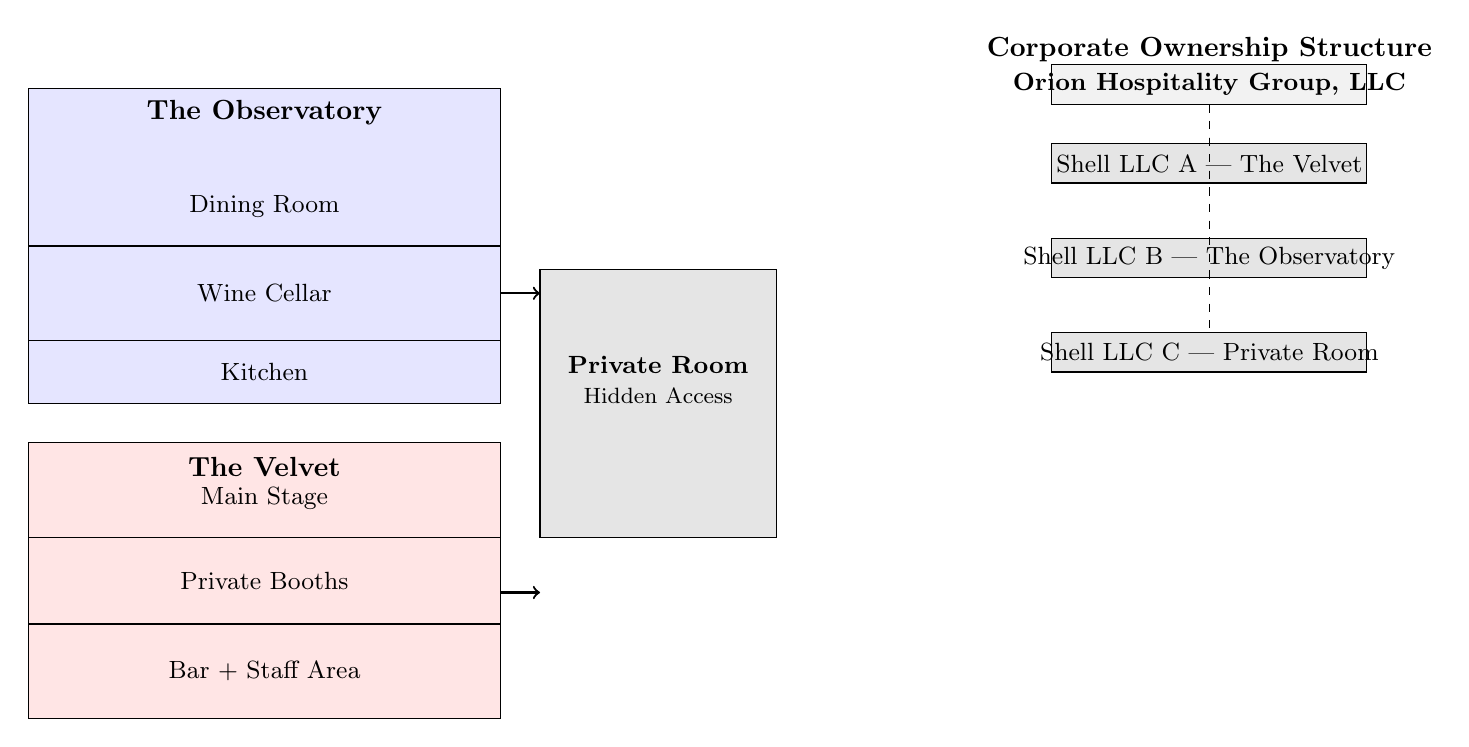
\begin{tikzpicture}[scale=1, font=\small]
  
    % === FLOOR PLAN ===
  
    % The Observatory — 1st Floor Layout
    \draw[fill=blue!10] (0,4) rectangle (6,8); % Restaurant
    \node[font=\bfseries] at (3,7.7) {The Observatory};
    \draw (0,6) -- (6,6); % Divider line
    \node at (3,6.5) {Dining Room};
    \draw (0,4.8) -- (6,4.8);
    \node at (3,5.4) {Wine Cellar};
    \node at (3,4.4) {Kitchen};
  
    % The Velvet — Basement Layout
    \draw[fill=red!10] (0,0) rectangle (6,3.5); % Club
    \node[font=\bfseries] at (3,3.2) {The Velvet};
    \draw (0,2.3) -- (6,2.3);
    \node at (3,2.8) {Main Stage};
    \draw (0,1.2) -- (6,1.2);
    \node at (3,1.75) {Private Booths};
    \node at (3,0.6) {Bar + Staff Area};
  
    % Shared Private Room
    \draw[fill=gray!20] (6.5,2.3) rectangle (9.5,5.7); 
    \node[align=center] at (8,4.3) {\textbf{Private Room}\\\footnotesize Hidden Access};
  
    % Entry arrows to Private Room
    \draw[->, thick] (6,5.4) -- (6.5,5.4); % From wine cellar
    \draw[->, thick] (6,1.6) -- (6.5,1.6); % From booths
  
    % === CORPORATE STRUCTURE ===
    \node[font=\bfseries] at (15,8.5) {Corporate Ownership Structure};
  
    % Parent company
    \draw[fill=black!5] (13,7.8) rectangle (17,8.3);
    \node at (15,8.05) {\textbf{Orion Hospitality Group, LLC}};
  
    % Shells
    \draw[fill=black!10] (13,6.8) rectangle (17,7.3);
    \node at (15,7.05) {Shell LLC A — The Velvet};
  
    \draw[fill=black!10] (13,5.6) rectangle (17,6.1);
    \node at (15,5.85) {Shell LLC B — The Observatory};
  
    \draw[fill=black!10] (13,4.4) rectangle (17,4.9);
    \node at (15,4.65) {Shell LLC C — Private Room};
  
    % Optional: connecting lines (just visual)
    \draw[dashed] (15,7.8) -- (15,7.3);
    \draw[dashed] (15,7.8) -- (15,6.1);
    \draw[dashed] (15,7.8) -- (15,4.9);
  
  \end{tikzpicture}
  \caption{
    Architectural floor plan of The Observatory (restaurant), The Velvet (club), and a hidden shared private 
    room — all legally separated by distinct shell LLCs but operated under a single parent entity.
  }
\end{figure}
  
\medskip 

The girls were not staff. But they were not exactly guests, either. The girls were just close 
enough to blur the line, and just far enough to keep anything that happened off the books.

The room itself was equal parts seduction and strategy. On the far side, a 
large circular bed 
slowly revolved under soft amber lights, not fast enough to draw attention, but just enough to suggest movement even when no 
one was on it. Opposite that, a narrow staircase led up to a small balcony lounge with low armchairs and a view that looked 
down over everything: the bed, the tables, and the guests. From up there, the whole scene played like theater.

Beneath the balcony sat a tastefully integrated dancer’s pole that was polished to a mirror finish.
Between the pole and the bed, a row of dark walnut tables offered just enough space for a whiskey flight.
Leather-backed chairs, matte black sugar trays, flickering votives completed the setup, and evoked a high-end coffee shop 
more than a club. It gave cover to whatever the guests chose to call the evening.


After dessert, it wasn’t uncommon for the night to 
migrate there.  Sometimes the wives joined. Sometimes they didn’t.  Sometimes 
they brought their own guests.  On the expense report, it was just a dinner.  It was just a networking event.  
It was just a hospitality line item.  But everyone understood. What happened in the private room wasn’t on the receipt.  
But it was part of the bargain.

If anything compromising happened in that room — a lapse in judgment, a moment of indulgence, a scene that didn’t belong 
in a compliance report — it wouldn’t trace back to the restaurant or the club. Not directly.

The layout made that possible. And so did the paperwork.

The private room acted like a firewall. It was where someone could have a ``business dinner'', and no one would ask questions. 
The circular bed wasn’t just for show, and the mirrored ceiling above it wasn’t an accident. 
Security staff knew where to turn the cameras, and the exit to the Velvet was marked only from the inside. 

\medskip

\begin{TechnicalSidebar}{Significance of a Shell LLC Leasing the Private Room}

  The decision to lease the private room under a shell company wasn’t just legal 
  hygiene. It was structural intent.

  \medskip
  
  First, it created containment. If anything controversial or reputationally toxic happened behind those doors — 
  a lapse in decorum, a breach of ethics, even a crime — liability wouldn’t touch the restaurant or the club. Not 
  directly. On paper, the room belonged to a “private event services firm,” a neutral tenant with no obvious 
  connection to adult entertainment or fine dining. To regulators, auditors, or journalists, the room became a 
  dead end in the org chart.

  \medskip
  
  That insulation granted flexibility. The space could serve multiple roles depending on who was asking. From the 
  restaurant’s side, it might be described as a wine cellar annex or executive dining suite. From the club’s side, 
  it could be pitched as VIP overflow, though never formally listed as part of the venue. And if the conversation 
  was too delicate for either brand to claim, the room could simply be leased out to “external partners” — a 
  euphemism everyone understood.

  \medskip
  
  Then came the deniability. If subpoenas arrived or FOIA requests were filed, staff could answer with complete 
  honesty: that room wasn’t under their control. Access logs, contracts, and invitations all pointed elsewhere. 
  The ambiguity wasn’t a flaw in the structure. It was the feature.

  \medskip
  
  But the real power came in access management. Because the room sat in the jurisdiction of a separate LLC, so 
  did its entry permissions. Key cards, security footage, guest lists were all handled through a different custodial 
  layer. It became a liminal space: technically private, legally detached, and socially malleable. Only insiders 
  understood how fluid the boundary really was.

  \medskip
  
  And finally, there was the financial dimension. A standalone LLC could receive funding through hospitality budgets, 
  bill clients under consulting fees, or depreciate the cost of “client engagement.” Revenues could be rerouted. 
  Expenses could be categorized to fit the desired story. And most importantly, any paper trail would read like a 
  footnote in someone else’s ledger.

  \medskip
  
  This wasn’t just about hiding things. It was about structuring optionality. It was not secrecy for its own sake, 
  but mobility. The kind of mobility that made denial credible, audit trails blurry, and influence hard to trace.
  
\end{TechnicalSidebar}

\medskip

\subsection{The Architecture of Mutual Compromise}


But sex wasn’t the only reason the room existed. That was just the cover.

Its real value came when that same room became the setting for off-calendar meetings. Regulators took calls on encrypted 
phones while pretty girls sat on their laps. Vendors pitched exclusivity clauses without lawyers present. A government 
liaison once reviewed a demo on a tablet between dances.

By law, to avoid conflicts of interest, to preserve impartiality, and to maintain the appearance of independence,
there are situations where \textbf{regulators, auditors, and clients aren’t allowed to share the same room outside
official business}.

But no statute prohibits a regulator from dining at the Observatory, or a client from entering the Velvet. And if they 
happened to meet in the private room? Well, that was just coincidence.

And everyone who entered the room had skin in the game. The cameras weren’t official, but the girls had seen your face. No 
one said it aloud, but the room made sure that what happened there stayed off the record. It made people speak differently. 
It made them speak more candidly. And it made them more open to compromise.


It wasn’t unusual for a portfolio to be rebalanced while someone’s wife “entertained” multiple men on stage as part of 
the deal itself. For those in the know, her ``performance'' 
\footnote{Her performance carried implications far beyond the surface. It wasn’t just erotic; it was managerial.
Iceberg Slim in his autobiography ``PIMP: My Life'' once described how his mentor taught him how to ``keep a bitch under 
control'': beat her, then give her a cold bath. The comfort
that follows pain, he said, rewires the loyalty. ``She'll be so thankful for the comfort that she'll forget that you were 
the one who hurt her'', he said. In BDSM, they call it ``aftercare''.
In elite circles, they call it ``hospitality''. Either way, it’s the same logic: control wrapped in tenderness.
This wasn’t indulgence; it was choreography. A performance staged to remind the room who offered warmth,
and who could take it away. A performance staged to remind the room who could hurt you, and who could help you.
What’s ``abuse'' when you’re poor becomes ``ritual'' when you’re rich.
What’s trashy in public becomes classy behind French doors.}
was a message disguised as a spectacle to prove her husband's loyalty and compliance.

That was the real purpose: deniability and leverage.

Because in rooms like this, the real power wasn’t in what was said.  It was in what no one dared to say aloud.

\medskip

\begin{figure}[H]
  \centering

  % === First row ===
  \begin{subfigure}[t]{0.45\textwidth}
  \centering
  \begin{tikzpicture}
    \comicpanel{0}{0}
      {Old Pimp}
      {Young Pimp}
      {To keep her loyal, hurt her then be the one to comfort her. She'll call it kindness.}
      {(-0.6,-0.6)}
  \end{tikzpicture}
  \caption*{The lesson: control delivered as a kindness.}
  \end{subfigure}
  \hfill
  \begin{subfigure}[t]{0.45\textwidth}
  \centering
  \begin{tikzpicture}
    \comicpanel{0}{0}
      {Old Pimp}
      {Young Pimp}
      {OK. But what will the cops call it?}
      {(0.6,-0.6)}
  \end{tikzpicture}
  \caption*{The suspicion: wondering what name gets printed on the charge sheet.}
  \end{subfigure}

  \vspace{1em}

  % === Second row ===
  \begin{subfigure}[t]{0.45\textwidth}
  \centering
  \begin{tikzpicture}
    \comicpanel{0}{0}
      {Venture Hostess}
      {Private Guest}
      {His wife fucked the whole room. Then they whispered to her, ``You were radiant.''}
      {(-0.6,-0.6)}
  \end{tikzpicture}
  \caption*{The reenactment: how to package power plays as premium hospitality.}
  \end{subfigure}
  \hfill
  \begin{subfigure}[t]{0.45\textwidth}
  \centering
  \begin{tikzpicture}
    \comicpanel{0}{0}
      {Venture Hostess}
      {Private Guest}
      {Is that aftercare... or just classier pimping?}
      {(0.6,-0.6)}
  \end{tikzpicture}
  \caption*{The question: when power hides behind legal definitions.}
  \end{subfigure}

  \caption*{If you file it under ``team development,'' you can make pimping a corporate expense.}
\end{figure}

\medskip

\begin{PhilosophicalSidebar}{The Thumbscrew Principle --- Leveraging Mutual Compromise as Insurance}
In high-stakes consulting, reputational risk isn’t always mitigated through compliance—it’s mitigated through 
\textbf{mutual compromise}.  

\medskip

\textbf{Law 33} from \textit{The 48 Laws of Power} explains the underlying psychology:  

\begin{quote}
Discover each man’s thumbscrew.
\end{quote}

In this context, the thumbscrew isn’t leverage from blackmail—it’s the leverage of \textbf{co-participation}. 
You don’t need to threaten exposure if you’ve already pulled them into the same compromising behaviors. Every 
indulgence, every ethical lapse, and every blurred boundary is an insurance policy.  

\begin{quote}
If everyone’s hands are dirty, no one wants to wash them first.
\end{quote}
\end{PhilosophicalSidebar}

\medskip



  



The brilliance wasn’t coercion.  The brilliance was \textbf{slow entanglement}. 
Entanglement so gradual that no single step felt like a compromise.

The Observatory wasn’t a trap door.  It was a funnel lined in velvet.

\begin{quote}
  The real contract wasn’t signed on paper.  The real contract was the months of rooms you shared.
\end{quote}

Hart’s brilliance wasn’t creating leverage over people. It was creating an ecosystem where 
\textbf{everyone had leverage on everyone else}, and thus, no one dared pull the thread.

\medskip

\begin{HistoricalSidebar}{The Broadcom ``Pond'': Henry Nicholas III and the Velvet Trap}

  In the late 1990s and 2000s, tech billionaire \textbf{Henry Nicholas III}, co-founder of Broadcom, wasn’t just making 
  semiconductor chips—he was making headlines for a hidden world beneath his empire.

  \medskip
  
  According to federal prosecutors and court filings, Nicholas built an underground lair beneath his Laguna Niguel warehouse: 
  a secret cave outfitted with a Jacuzzi for six, an \$18{,}000 handcrafted bar, and an Oriental-themed parlor adorned 
  with rugs, statues, and a four-foot Medusa figure. They called it \textbf{“The Ponderosa”} or \textbf{“The Pond.”} 
  Behind a hidden library wall in his mansion, another secret tunnel led to an underground sports bar and recording 
  studio.

  \medskip
  
  But these weren’t just eccentric architectural choices. These were spaces designed for what court filings described as 
  \textbf{marathon drug-fueled orgies}, mixing cocaine, ecstasy, nitrous oxide, prostitutes, and music from Led Zeppelin 
  and Phil Collins in a surreal, days-long bacchanal.

  \medskip
  
  A former employee described the parties: a black box of cocaine sat atop the bar next to a grinder for crushing rocks 
  into powder. A bartender—whom Nicholas had personally sent to bartending school to perfect his favorite cocktail, the 
  \emph{grasshopper}—served guests as they inhaled “whippets” from metal canisters, later replaced by a full nitrous 
  tank when the guests complained the canisters were too cold.

  \medskip
  
  The parties were exclusive, indulgent, and heavily curated. Clients, employees, regulators, and other VIPs were invited 
  to ``network''. A former assistant alleged he was forced to act as a drug courier and to make sure his "friends" were 
  entertained with prostitutes.

  \medskip
  
  When legal troubles surfaced, no formal charges of blackmail or hostage-taking emerged, but the \textbf{dynamic of 
  mutual compromise was clear}:  

  \begin{quote}
    Everyone inside the cave had a stake in the silence.  Everyone left with something they couldn’t easily admit.  
  \end{quote}
  
  Nicholas didn’t need overt threats. The space itself was the leverage. Participation was the insurance policy.  

  \medskip
  
  And when a regulator, client, or associate later hesitated to follow his lead, the implication wasn’t spoken, but it 
  was understood:  \textit{“We were in the cave together.”}

  \medskip
  
  His case ended with dropped charges, plea deals, and no prison time. But the broader lesson lingers: Nicholas built 
  more than a secret room—he built a velvet trap, where the real power wasn’t what he held over others, but what they 
  already held over themselves.

  \medskip

  And the final irony?
  
  \medskip

  After years of drugs, prostitutes, and corruption swirling beneath the radar, what finally brought authorities to his 
  doorstep wasn’t the cave’s activities—it was a noise complaint from neighbors, triggered when Nicholas tried to expand 
  his secret sex dungeon without a building permit by hiring undocumented Mexican laborers to excavate it in secret.

  \begin{quote}
  ``The Pond'' survived the long arm of the law, but it couldn’t survive the long arm of the home owner's association.
  \end{quote}

\end{HistoricalSidebar}

\medskip

It wasn’t about written agreements, enforceable terms, or formal obligations. It was about weaving participants into a 
\textbf{mutual dependency of silence}, a tacit agreement built not on paper but on complicity.

Every invitation to an off-book dinner, every casual introduction to a “friend of the firm,” and every night where boundaries 
blurred wasn’t just a favor. It was a stitch in the fabric of a collective secret. A secret that tied everyone 
together in a web where exposure couldn’t be isolated. To expose anyone else was to expose yourself.

The genius of this ecosystem wasn’t overt coercion. It was self-reinforcing compliance. Once inside, no one wanted to 
be the first to speak. And no one wanted to be the first to walk away. Because leaving clean required admitting you were 
never clean.

This is the architecture of \textbf{distributed leverage}:  No single actor holds absolute power over the others because 
everyone holds just enough dirt to keep the group stable. It mirrors the principle of \emph{mutually assured destruction}, 
but at the level of reputation and informal loyalty rather than military force.

\medskip

\begin{PsychologicalSidebar}{Distributed Leverage and the Psychology of Pluralistic Ignorance}

  In 1931, social psychologist \textbf{Floyd Allport} first coined the term \emph{pluralistic ignorance} to describe a 
  curious phenomenon: a group of individuals might all privately disagree with a norm or practice, yet publicly uphold 
  it because they mistakenly believe everyone else supports it.
  \medskip

  Later, researchers like \textbf{Daniel Katz} and \textbf{Floyd Allport} expanded the concept through experimental 
  studies, showing how this false consensus effect sustains unethical or undesirable group behavior—not through overt 
  coercion, but through collective misperception.

  \medskip

  In Hart’s ecosystem, pluralistic ignorance wasn’t just an incidental byproduct—it was engineered.

  \medskip

  Each private dinner, each informal introduction, each blurry night of implicit favors created a shared assumption: 
  \textbf{“Everyone else is comfortable with this. Everyone else is playing along.”}

  \medskip

  But beneath the surface, many participants might have felt uneasy. The genius of the system was that no one could 
  tell. Silence became the default, not because everyone agreed, but because no one wanted to be the first to admit 
  discomfort.

  \medskip

  And with every silent nod, the ecosystem hardened. Each individual believed departure would mean revealing not just 
  their own doubts—but their own complicity.

  \medskip

  Psychologists studying pluralistic ignorance found that the longer such a norm persists unchallenged, the stronger 
  it feels --- even if privately, no one endorses it.

  \begin{quote}
    The brilliance of distributed leverage isn’t enforcing consensus.  It’s making each individual believe consensus 
    already exists.
  \end{quote}

\end{PsychologicalSidebar}

\medskip

Hart didn’t merely sell access. He didn’t merely sell deals. He sold membership in a system that rewrote the very 
rules of accountability.

\begin{quote}
  Because a cartel doesn’t need to control the market if it controls the consequences of leaving.
\end{quote}

And the more entangled you became, the harder it was to chart a path back to independence. Why? Because every bridge out 
had already been soaked in the gasoline of shared participation.

Hart’s real product wasn’t strategy, capital, or connections.  
Hart’s real product was the invisible web.  
\textbf{It was a structure where participation became the only viable strategy.}

\medskip

\begin{HistoricalSidebar}{Enron, Strip Club Lu, and the Audit that Never Happened}

  In the early 2000s, as the collapse of \textbf{Enron} shook global markets, a secondary casualty followed: 
  \textbf{Arthur Andersen}, once one of the “Big Five” accounting firms, disintegrated under the weight of 
  complicity.  

  \medskip
  
  The natural question lingered: \textit{How did the auditors miss it?}  

  \medskip
  
  Then the stories of \textbf{“Strip Club Lu”} surfaced.  
  
  \medskip
  
  Lu, an Enron executive, had become notorious across Houston’s nightlife scene. His nickname wasn’t ironic. 
  It was literal. Lu was known for throwing down so much cash at strip clubs that you couldn’t see the floor 
  under the dollar bills. And the best part?  \textbf{It was all expensed.}  

  \medskip
  
  Officially filed under “research,” Lu’s excursions weren’t solo adventures. He brought \textbf{clients}, 
  \textbf{partners}, and even \textbf{auditors} along for the ride. What began as networking spiraled into 
  bacchanals of absurd excess.  
  
  \medskip
  
  When the \textbf{SEC investigation} later combed through emails, they uncovered something even darker: 
  multiple warnings from Enron’s internal compliance officer, \textbf{Sherron Watkins}, and from other 
  executives like \textbf{David Skilling} (nicknamed “Skelleg” in internal memos), begging Lu to stop 
  using Enron’s offices for after-hours parties.  

  \medskip
  
  The emails weren’t vague: they referenced \textbf{orgies in the office with strippers}, documented 
  concerns about security footage, and outright pleas to stop turning corporate headquarters into a 
  late-night adult playground.  
  
  \medskip
  
  And yet, within the industry, everyone knew.  

  \medskip
  
  Stories about Enron’s “hospitality” weren’t whispered—they were \textbf{bragged about}. Competitors joked 
  about partnering with Enron just to enjoy the legendary parties. Visiting investment bankers told stories 
  of the corporate Amex being swiped for champagne fountains. And behind it all, Arthur Andersen’s auditors 
  kept signing off on the books.  
  
  \medskip
  
  The brilliance (if it can be called that) wasn’t a cover-up. It was \textbf{mutual indulgence}.  
  
  \begin{quote}
  When everyone’s at the party, no one wants to turn on the lights.
  \end{quote}
  
  Enron’s collapse wasn’t just a financial failure. It was a case study in what happens when complicity becomes 
  cultural currency, and reputational risk is managed through \textbf{mutual dirt}.  
  
  \begin{quote}
  The real audit wasn’t the one filed in the reports.  
  The real audit was the chain of silent approvals signed with every swipe of the card.
  \end{quote}
  
  In the end, Arthur Andersen didn’t fail because they didn’t know.  Arthur Andersen failed because they did.
  
\end{HistoricalSidebar}

\medskip

\subsection{Whiskey, Warmth, and the Weaponization of Yes}

That’s why Hart chose this room for the real conversation.  
Not because it was private.  
But because it was preloaded with consent.

Leather walls. No windows. A table just small enough to keep everyone close.  
And a bottle of Japanese whiskey in the center.

David sat across from him, with Paolo — the regulator liaison — at his side.  
And flanking them, always within reach, were the girls from the gentleman's club.

\medskip

\begin{PhilosophicalSidebar}{Regulatory Capture — When Oversight Learns to Speak Client}

  In theory, regulators exist to safeguard the public interest — ensuring that safety, transparency, and fairness 
  override private ambition.  
  But in practice, something quieter often unfolds: oversight doesn’t disappear. It \textit{assimilates}.  

  \medskip
  
  This is the essence of \textbf{regulatory capture}.

  \medskip
  
  Not bribery. Not threats.  
  Just proximity. Familiarity. The soft erosion of boundaries through shared incentives and shared vocabulary.
  
  \medskip
  
  \textbf{Paolo} wasn’t just a liaison. He was a translator.  
  The bridge between regulatory opacity and startup ambiguity.  
  He’d spent years mastering the dialect of both sides: how to phrase a model’s interpretability risk as a “technical 
  opacity window,” how to reframe edge-case failures as “innovation latitude.”
  
  \medskip
  
  Hart didn’t need Paolo to sign off.  
  He needed him to nod at the right moments.  
  To offer a “soft read” on which clauses might trigger scrutiny.  
  To hint at how far the edges of compliance could stretch without snapping.
  
  \medskip
  
  Officially, Paolo wasn’t allowed to shape deployment timelines.  
  Unofficially, he could signal just how much regulatory slack they had, and how quietly a deployment might slide 
  through under an innovation exemption.

  \medskip
  
  That’s why he was in the room.

  \medskip
  
  Not to approve.  
  Not to object.  
  But to observe. And later, to forget just enough of what he saw.
  
  \medskip
  
  This is how capture works:  
  Not through malice, but through \textbf{mutual alignment}.  
  The regulator begins to see the world not as it is, but as the client wants it to be.  
  What starts as interpretation becomes advocacy.  
  What starts as oversight becomes choreography.
  
  \begin{quote}
  The danger isn’t that the watchdog falls asleep.  
  It’s that he learns the pitch deck.
  \end{quote}
  
\end{PhilosophicalSidebar}

\medskip


One girl draped her arm casually over Hart’s shoulder. She brushed his lapel with a faux-absentminded touch.  
Another leaned in to refill David’s glass with her nails tapping lightly on the stem as she steadied it.  
The perfume shifted every time someone moved. He smelled musk, citrus, and smoke.  

It wasn’t a formal pitch. But it wasn’t casual either.

At the time, David didn’t question the setting.  
He chalked it up to Hart’s signature flair. The curated decadence. The blurred line between deal and indulgence.
It is what everyone came to expect.  

The room was just private enough to lower one’s guard, and just dim enough to dull consequence.  

The girls were warm, playful, and always half-involved. 

The girls gave the whole scene the texture of safety.  

The girls made it feel like no one would remember what was said, so long as no one wrote it down.

But later, he would understand.

\textit{This wasn’t just where the deal happened.}  

\textit{This was where something crossed a line.}

He didn’t sign a document that night.  
But he said something he shouldn’t have.  

He agreed to something he wasn’t ready for.  
Because he let the room decide for him.

And by the time he realized why Hart had chosen this room ---
with its erotic silence and curated distractions ---  
it was too late to walk it back.

“We’ve already routed exposure through the model at Arcadia,” he said, smiling. 
“It’s holding up beautifully under stress.”
Hart leaned back with one arm resting along the top of the table and the other wrapped around a 
glass of scotch that seemed never to empty. 

One of the girls giggled, not at the words, but at the warmth in Hart’s tone. She whispered something into his ear. 
But he didn’t break eye contact with David.

David said nothing. Not because he agreed. But because correcting Hart would have meant introducing friction. And the 
room had been designed to punish friction. Everything here was buffered: light, sound, and dissent.

A girl walked past and trailed her hand along the back of Paolo’s chair. Paolo didn’t flinch, either because he didn’t 
notice or because he knew not to.

Paolo turned to David. “Impressive,” he said. “So it’s in live deployment?”

David hesitated. Not because the answer was complicated, but because another woman had leaned gently against the edge 
of the table beside him. She let her fingers trail along his thigh, featherlight. It was more suggestion than touch. 
More strategy than affection.

“We’re...” David adjusted in his seat. “Finalizing interpretability for regulated clients. Some edge-case volatility 
around correlation breaks. But nothing that would preclude a limited pilot.”

He hated how the words sounded coming out of his mouth. It was technically true, but also incomplete. But the truth 
wasn’t the currency here.

Because by the time David realized it, they hadn’t just partnered with Centauri.

They’d been \textbf{acquired in all but paperwork}.

Another girl returned with drinks and slipped into the space beside Hart and David. She perched like a bird trained to rest on 
expensive shoulders. Her smile was more curated than warm.

“They’ve got two desks looking to replace their quant overlays by Q3,” Paolo said casually. “If the stability’s there, 
you could slip it in under their innovation mandate.”

David looked up. He should’ve said no. He should’ve said “Q4 at the earliest.” He should’ve said “We haven’t passed 
adversarial stress.”

But instead, he nodded. Not because the system was ready, but because the social machinery was already in motion. 
He was no longer being asked to evaluate a deployment schedule.

He was being asked if he belonged.

\begin{quote}
Paolo expects this. Paolo was brought into the loop with you. Paolo smiled at you across the table while the 
deal was forming.
\end{quote}

To push back now would not be a technical objection. It would be a social betrayal.

“That’s doable,” David said.

Hart raised his glass. The girl beside him clinked hers against his without being asked.

“To velocity,” Hart said smoothly, “and to teams that don’t wait for permission.”

They all clinked glasses.  
Paolo smiled.  
The woman beside David leaned close enough to break the threshold where lapse in judgement 
turns into impulse. So when she leaned in, he mistook her presence for peace.

And with a nod, a sip, a sentence he couldn’t take back,  
and a moment of silence that smelled like perfume...
David had just approved the deployment.

Then David swallowed his scotch like a confession.
Not to release it, but to trap it somewhere deeper.

But the burn wasn’t enough.

That's why when she kissed him, he kissed her back.

But he did not kiss her out of want.

He kissed her to forget --- for the moment --- that this burden was his alone to carry.

It was not desire. And it was not connection. 

It was anesthesia with a pulse.

\medskip

\begin{PhilosophicalSidebar}{Professional Ethics, Conflict of Interest, and the Structure of Trust}

  At the heart of professional ethics lies not morality, but preservation. Professional ethics is not about individuals
  morality, but about the profession itself.

  \medskip
  
  Engineers, doctors, and lawyers are held to a higher standard not because they are inherently more virtuous, but because 
  the public must believe they are. Without trust in the profession, the system that relies on them collapses.

  \medskip
  
  
  This is why a doctor is delicensed for intentionally harming a patient, even if they believe it’s ``for their own good.''
  This is why a lawyer is disbarred for lying to a judge, even if it secures the client’s victory. The damage is not just to 
  the case, but to the credibility of the legal system itself. The punishment isn't about wrongdoing: it’s about maintaining 
  the fiction that professionals serve truth, and not their employer.

  \medskip
  
  
  Across industries, entire regulatory architectures are built to separate power from practice. Medical administrators may 
  oversee budgets, but they are legally barred from dictating medical decisions. Project managers handle scope and timelines, but 
  not engineering decisions. Corporate lawyers can direct business strategy, but cannot ignore legal obligations without 
  putting the company — and the entire profession — at risk.

  \medskip
  
  
  In situations of conflict, a professional must invoke a higher loyalty: \textit{professional ethics}. A doctor must say, 
  ``I cannot do that, even if the CEO asks.'' A lawyer must say, ``I serve the law first.'' An engineer must say, ``That shortcut 
  would compromise safety.'' Their oath binds them not to the client, but to the discipline itself.

  \medskip
  
  In essence: \textbf{Ethics begins where control ends.}

  \medskip
  
  To protect a profession, you must give its members the authority to say no, and the obligation to mean it.
  
\end{PhilosophicalSidebar}




